\documentclass{article}% use option titlepage to get the title on a page of its own.
%\usepackage{blindtext}
\usepackage{listings}
\usepackage{tikz}
\usepackage{graphicx}
\graphicspath{{./images/}}
\title{Crearea retelelor de sortare folosind retele neuronale recurente}

\date{2018\\ Iulie}

\author{Danila Marius Cristian}

\begin{document}

\maketitle

\section{Retele de sortare, prezentare}

\noindent Formal, definim o retea de sortare de dimensiune $N$ ca fiind o colectie de $N$ fire si $M$ comparatori. Comparatorii \noindent au rolul de a interschimba doua elemente aflate pe fire diferite, elementele trebuie sa satisfaca un predicat $P$ \noindent astfel incat la finalul aplicarii secventei de comparatori pe elementele aflate in retea sa obtinem o secventa aflata in ordine.

\noindent Schematic, ilustram o retea de sortare cu 4 fire astfel: \break
\begin{center}
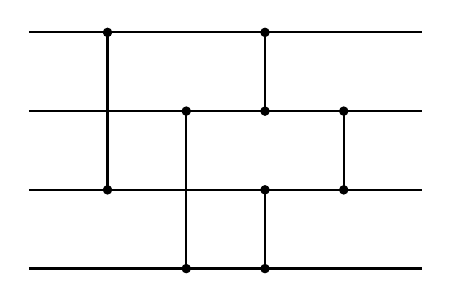
\begin{tikzpicture}
%\fill [gray!15] (1.5,1.5) -- (2.5,1.5) -- (2.5,2.5) -- (1.5,2.5) -- cycle;
\foreach \a in {1,...,4}
  \draw[thick] (0,\a) -- ++(5,0);
\foreach \x in {{1,2},{1,4},{2,1},{2,3},{3,1},{3,2},{3,3},{3,4},{4,2},{4,3}}
  \filldraw (\x) circle (1.5pt);
\draw[thick] (1,4) -- (1,2);
\draw[thick] (2,1) -- (2,3);
\draw[thick] (3,1) -- (3,2);
\draw[thick] (3,3) -- (3,4);
\draw[thick] (4,2) -- (4,3);
\end{tikzpicture}
\end{center}


\subsection{Metode imperative de generare a retelelor de sortare}

Exista mai multe metode imperative pentru a genera o retea de sortare. Cele mai usoare modalitati sunt de a generea o 
retea bazata pe algoritmii de sortare bubble sort si insertion sort. In cazul primei optiuni se adauga un comparator intre
firele $0$ si $1$, $1$ si $2$, ..., $n-1$ si $n$. Se reaia procesul de creere a comparatorilor inserand un comparator intre $0$ si $1$, ..., $n-2$ si $n-1$. Se repeta aceasta procedura de creere a comparatorilor pana la pasul in care inseram un singur comparator intre firele $0$ si $1$.

In cazul unei insertion sorting network, o retea bazata pe insertion sort procesul este similar, singura diferenta este ca buclele de creare a comparatorilor sunt in ordine inversa fata de metoda precedenta. Astfel, prima data se creeaza un comparator 
intre firul $0$ si $1$. Se creeaza un comparator intre $0$ si $1$, $2$. Pana cand se ajunge la pasul in care se generaza un comparator intre $0$ si $1$, ..., $n-1$ si $n$. 

Un exemplu de bubble sorting network:
\begin{center}
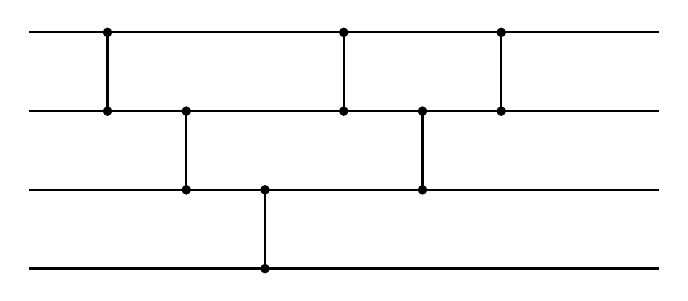
\begin{tikzpicture}
%\fill [gray!15] (1.5,1.5) -- (2.5,1.5) -- (2.5,2.5) -- (1.5,2.5) -- cycle;
\foreach \a in {1,...,4}
  \draw[thick] (0,\a) -- ++(8,0);
\foreach \x in {{1,4},{1,3}, {2,3},{2,2},{3,2},{3,1},{4,4},{4,3},{5,3},{5, 2}, {6, 3}, {6, 4}}
  \filldraw (\x) circle (1.5pt);
\draw[thick] (1,4) -- (1,3);
\draw[thick] (2,3) -- (2,2);
\draw[thick] (3,2) -- (3,1);
\draw[thick] (4,4) -- (4,3);
\draw[thick] (5,3) -- (5,2);
\draw[thick] (6,4) -- (6,3);

\end{tikzpicture}
\end{center}

Un exemplu de insertion sorting network:

\begin{center}
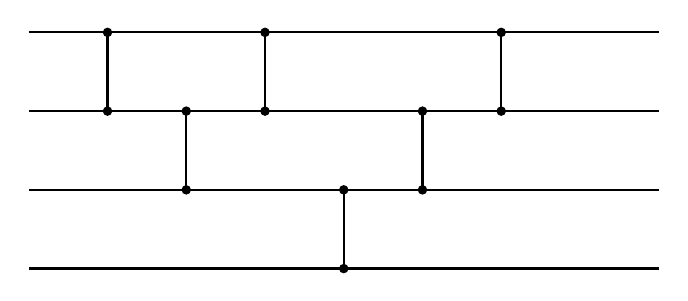
\begin{tikzpicture}
%\fill [gray!15] (1.5,1.5) -- (2.5,1.5) -- (2.5,2.5) -- (1.5,2.5) -- cycle;
\foreach \a in {1,...,4}
  \draw[thick] (0,\a) -- ++(8,0);
\foreach \x in {{1,4},{1,3}, {3,4},{3,3},{2,3},{2,2},{4,2},{4,1},{5,3},{5, 2}, {6, 3}, {6, 4}}
  \filldraw (\x) circle (1.5pt);
\draw[thick] (1,4) -- (1,3);
\draw[thick] (3,4) -- (3,3);
\draw[thick] (2,3) -- (2,2);
\draw[thick] (4,2) -- (4,1);
\draw[thick] (5,3) -- (5,2);
\draw[thick] (6,4) -- (6,3);

\end{tikzpicture}
\end{center}

Algoritmul imperativ pe care l-am folosit pentru a genera un bubble sorting network este:
\begin{lstlisting}
    def bubble_sorter(n):
        if n <= 1:
            return []

        ret_val = []
        for i in range(0, n - 1):
            ret_val.append((i, i + 1))
        ret_val += self.dummy_sorter(n - 1)
        return ret_val
\end{lstlisting}
Pentru un numar de fire dat, $n$, generam lista de comparatori, adica conexiunile dintre firele din retea.
%\break

    Aceste arhitecturi de retele de sortare nu sunt optimale si vor sorta un sir de numere ca input in timp
$O(n^2)$. Retelele optimale si cele mai des folosite in practica sunt bazate pe algoritmul bitonic sort, acestea ating complexitate de $O(nlog^(n))$. Insa motivul pentru care am prezentat bubble sorting network si insertion sorting network este
ca bazandu-ne pe acesti algoritmi am generat datele de antrenament pentru modelul dezvoltat.

\section{Retele neuronale, prezentare}

Retelele neuronale reprezinta o ramura a inteligentei artificiale. Sunt modele abstracte ce incearca sa simuleze creierul uman
in modul de intercationare cu natura. O retea neuronala este compusa din neuroni artificiali. Neuronii artificiali din retea sunt dispusi pe mai multe straturi. Din exterior le putem vedea ca pe un black box conectat la un strat de neuroni de input, responabil de preluarea inputlui si la un strat de neuroni de output, responsabil pentru a genera outputul. In functie de neuronii din stratul de output care se vor activa se decodifica rezultatul produs de retea.

\subsection{Arhitecturi de retele neuronale}
Retelele neuronale convolutionale sunt modele simple, proiectate sa primeasca un set de input fix si sa produca un set output output de marime fixa. In practica, acest tip de retele sunt ideale pentru computer vision. Sunt mult mai eficiente din punct de vedere al resurselor consumate la sarcini precum recunoasterea de obiecte in imagini. 

Retelele neuronale recurente se deosebesc de cele convolutionale prin posibilitatea de a primi un set de input variabil si a produce un set de output variabil. In practica se folosesc la procesarea limbajului natural. Acest tip de retele neuronale sunt ideale si pentru rezolvarea problemei de generare a retelelor de sortare, intrucat putem codifica numarul de fire din retea ca o secventa de lungime variabila, iar rezultatul, respectiv setul de comparatori pentru numarul de fire dat poate varia. Pe langa aceste considerente, acest tip de retele contin si o memorie atasata.

Un caz particular de retele neuronale recurente sunt *masinile turing neurale*. Acestea fiind optimizate in a invata algoritmi imperativi simpli. Un exemplu ar fi problema sortarii, rezolvata in mod traditional cu un algoritm imperativ poate fi rezolvata folosind acest tip de retele. Pentru aceasta, reteaua va primi ca input tuple de forma $(X, Y)$. Unde $X$ reprezinta un sir de numere aflate in ordine random, iar $Y$ reprezinta varianta sortata a sirului $X$ cu un algoritm imperativ de sortare. Odata antrenata pe un set suficient de mare de date de acest fel, modelul va invata practic sa aplice algoritmul de sortare folosit pe componenta $Y$. 

Motivul prezentarii scenariului de mai sus este ca hiperparametrii si structura straturilor de neuroni dintr-o retea de neuronala folosita la sortarea de numere sunt similari in proportie foarte mare cu cei din reteaua proiectata sa genereze retele de sortare.

\section{Tehnologii folosite}


\section{Descrierea solutiei}
Solutia problemei consta intr-un model antrenat pe un set de date produs de un algoritm imperativ de generare a retelelor de tip bubble sorting network si insertion sorting network. Peste modele generate avem o interfata web se permite vizualizarea in browser a retelei generate.

Arhitectura proiectului este:

\begin{center}
\includegraphics[scale=0.8]{architecture}
\end{center}

Arhitectural, avem un server web care ii trimite clientului codul interfeti grafice folosite la reprezentarea inputului pentru un numar dat de fire. Utilizatorul va alege ca input numarul de fire folosit si se va realiza un request ajax in spate cate serverul web. Serverul se conecteaza printr-un socket la model manager, ce coordoneaza cele doua modele antrenate si va trimite serverului prin socket comparatorii generati, in functie de modelul ales de utilizator. Serverul trmite la client comparatorii, iar clientul creeaza diagrama retelei respective.

\subsection{Arhitectura modelului}

Modelul este un "Neural Turing Machine". Pentru constructia modelului am folosit in spate un framework numit ntm-lasage, optimizat pentru crearea de modele de acest fel. Se abstractizeaza in acest fel detalii de implementare. 

Modelul contine o memorie cu un layout de $1024$x$160$ celule. Ca functie de loss am folosit crossentropia binara, pentru ca intern numerele ce vin ca input in model sunt reprezentate ca siruri binare.

Procesul de backpropagation este abstractizat de model. Actualizarea weighturilor din retea este optimizata cu rmsprop.
Datele de antrenament sunt procesate de retea in batchuri de 1.

Structura inputului retelei este de un vector de 9 elemente ce reprezinta codificarea in binar a numarului de fire din retea. Outputul retelei este un vector tridimensional cu $2*numar\_comparatori$ elemente. Elementele din vector sunt semantic grupate 2 cate 2, codificate ca un sir de biti, si reprezinta pozitiile comparatorilor din retea. 

\subsection{Antrenarea modelului}

Modelul ce genereaza retele bubble sorter a fost antrenat pe un set de input 1000 de elemente, pe numere mai mari de atat timpul necesar finalizarii procesului de antrenament devine foarte mare. Datele din setul de antrenament au fost generate conform algoritmului:
\begin{lstlisting}
    def bubble_sorter(n):
        if n <= 1:
            return []

        ret_val = []
        for i in range(0, n - 1):
            ret_val.append((i, i + 1))
        ret_val += self.dummy_sorter(n - 1)
        return ret_val
\end{lstlisting}

si arata astfel pentru un set de antrenament de 5 elemente:

\begin{lstlisting}
[2, [(0, 1)]]
[3, [(0, 1), (1, 2), (0, 1)]]
[4, [(0, 1), (1, 2), (2, 3), (0, 1), 
	(1, 2), (0, 1)]]
[5, [(0, 1), (1, 2), (2, 3), (3, 4), 
	(0, 1), (1, 2), (2, 3), (0, 1), (1, 2), (0, 1)]]
[6, [(0, 1), (1, 2), (2, 3), (3, 4), 
	(4, 5), (0, 1), (1, 2), (2, 3), 
	(3, 4), (0, 1), (1, 2), (2, 3), (0, 1), (1, 2), (0, 1)]]
\end{lstlisting}



\end{document}
